\documentclass[12pt,a4paper]{article}

\usepackage{epcc}
\usepackage{graphicx}
\usepackage{listings}
\usepackage{color}
\usepackage{amsmath}
\usepackage{subfig}
\usepackage{tabu}
\usepackage{array}
\usepackage{multirow}

\definecolor{mygreen}{rgb}{0,0.6,0}
\definecolor{mygray}{rgb}{0.5,0.5,0.5}
\definecolor{mymauve}{rgb}{0.58,0,0.82}

\usepackage{hyperref}
\hypersetup{
	colorlinks=true, %set true if you want colored links
	linkcolor=black,  %choose some color if you want links to stand out
}

\newcommand{\sectionVspacing}{\vspace{15pt}}

\begin{document}

\title{Message Passing Programming Coursework Assignment}
\author{Exam number B136013}
\date{\today}

\makeEPCCtitle

\thispagestyle{empty}

\newpage
\clearpage

\tableofcontents

\newpage
\clearpage

\section{Introduction}
	The goal is to solve an image processing problem. It uses a two-dimensional domain decomposition in order to split the workload to the active processes. To achieve this we use MPI communication protocol for process communication. This approach arises a variety of challenges that need to be addressed, such as communication and decomposition.

\sectionVspacing

\section{Project Description}
  The project takes as input a file that can be reconstructed to a greyscale image using a simple edge-detection algorithm. The mathematical model to reconstruct the image is\\
  \begin{equation}
  edge_{i, j} = image_{i-1, j} + image_{i+1, j} + image_{i, j-1} + image_{i, j+1} - 4*image_{i, j}
  \end{equation}
  There are a variety of project requirements in order to produce a correct output. There are fixed “sawtooth” boundary conditions in the horizontal direction. In addition, there are periodic boundary conditions in the vertical direction. This means that when a top process performs halo swap to fill the upper edge of the local table it receives it from the according to bottom process.\\
  Another specification is the terminate condition. The main loop of image reconstruction should finish when the maximum difference of a pixel in the image between the old and the value it's insignificant. This means that after some iterations when the produced image has not drastic variations from the previous the loop should be terminated.

\sectionVspacing

\section{Design Analysis}
	The design and control flow of the project is basically the same as the case study with a different implementation. The implementation of the project uses mainly the basic functions of the MPI API. Some of these features perform non-blocking communication, create a virtual topology and use derived types.

    \subsection{Initialization}
      In the initialization phase, MPI\_Init, MPI\_Comm\_rank and MPI\_Comm\_size functions are called to establish the communication for the active processes and for each process to learn its place in this network. Then program does a series of tasks

      \begin{enumerate}
        \item Reads the input image
        \item Decomposes of the problem
        \item Creates the virtual topology
        \item Discovers the topology
        \item Creates the Derived Types
        \item Allocates and Initializes the buffers
      \end{enumerate}

      \paragraph{Input}
			   The input of this experiment is an edge image and the number of process that are required to solve the problem. Every process reads the size of the input image but only the master process reads the raw data and stores it to its masterbuffer.

      \paragraph{Decomposition}
        In general, the algorithm has been designed to deal with any number of processes even for the occasion that they are not exactly divisible by the matrix size. The approach that we chose is that the border processes are going to deal with the extra workload. Decomposition process produces the size of the problem each process has to solve.

      \paragraph{Virtual Topology}
        In terms of the produced virtual topology, the main function was MPI\_Cart\_create that creates the new 2 dimension topology. Reorder of the given processes to the new topology is permited for optimazation reasons.

      \paragraph{Discover Topology}
        In this phase, it is necessary for each process to discover its place in the virtual topology and a new data structure called Cart\_Info. Cart\_Info contains all of the information a process needs to know when it comes to communication without the extra overhead of calling MPI functions to obtain these information on repeat. These information are the

      \begin{itemize}
			  \item World rank
			  \item MPI\_Comm of the virtual topology
			  \item World size
			  \item Its coordinates
			  \item Virtual topology's dimensions
			  \item The world ranks of its neghbours
			\end{itemize}

			In addition, methods like MPI\_Cart\_coords and MPI\_Cart\_rank have been used to identify the neighbor's ranks or coordinates. We have to say at this point that if a neighbour doen't exist it is set a MPI\_PROC\_NULL which helps as to avoid condition statements in the send functions.

        \paragraph{Derived Types}
            In order to reduce the code volume and avoid unnecessary memory allocations derived types are used extensively. Derived types such as row, column, and table are declared once in the main function. MPI\_Type\_vector has been the function that creates these derived types. Derived Types are used in the communication phase like the non-blocking functions. Their main goal is to avoid memory copies for the send and receive buffer. What we managed to is to read and write directly from and to the target buffers. As we mentioned before our Decomposition may assign different problem sizes to the process. In order to keep up code in a generic form, different implementations for the derived types have been the tool to address this issue.

        \paragraph{Buffers}
			Once we gathered these information we are able to dynamically allocate and initialize our buffers. All of the processes allocate the necessary buffers for the calculations using the sizes that decomposition phase has ordered. After that, the old buffer is initilized with the white (255) value. The boundary conditions are applied. To be more specific, if the worker has been assigned a part of the image which belongs to the left or right side, then sawtooth values are computed and stored.

    \subsection{Scatter}
        At this point the data exchange takes place. The master scatters the image which is stored in the masterbuffer directly to the edge buffers of the workers. Like in all of the communucation processes MPI\_Isend and MPI\_Irecv functions are used accordingly. More of the communication phase will be explained in the following section.

    \subsection{Calculation}
        At this point the main loop is ready to start. The calculation phase is decomposed as followed
        \begin{enumerate}
          \item Halo swaps are sent to the neighbors
          \item The middle calculations are computed (excluding borders)
          \item The program waits to the halo swaps and then calculate the borders
          \item Every 100 iteration, the average pixel is logged and the program checks if the loop can be terminated
          \item The new buffer is overwritten to the old one
          \item Step 1 is executed again
        \end{enumerate}

        \paragraph{Periodic Checks}
        	As mentioned before, at specific intervals in the loop the algorithm does some extra work. This work includes the logging of the average pixel's value. A Tab Seperated Value (TSV) file is generated to store this information. In addition a function is called to check if the execution can stop, which is the only way to exit the loop. This method checks the maximum difference between the pixels and if this value is below 0.1 for each of them the process is stopped. We have to point out that intervals have been set to 100 loop iterations as a design desicion. In extension MPI\_Allreduce function has been used twice in the periodic checks. First, to calculate the average pixel value which is part of the Output. Second, to calculate the max difference of the pixels.

        \paragraph{Communication}
            The corestone of the communication process are the MPI\_Isend and MPI\_Irecv functions. These methods are used for the halo swaps which are necessary for the calculations and the custom Scatter and Gather mechanisms. In the end of each of these procedures the program calls the MPI\_Wait function to ensure that there are not ongoing communications so the algorithm can resume its execution.

    \subsection{Gather}
    	Using the same tools as Scatter, Gather process is implemented, only in the opposite direction. The master gathers all of the old buffers and reconstructs the masterbuffer which will be written to the new output image.

    \subsection{Finalization}
    	The main job is done now the master process has gathered the calculated results. It will create the necessary files and store the logged information. To be more specific, the output are

      \begin{itemize}
		    \item A new reconstructed image
		    \item A TSV file that contains the input file, number of processes and average iteration running time (ms)
		  \end{itemize}

    	In the end each process will free the allocated buffers and call MPI\_Finalize function to end properly the communication between the processes.

\sectionVspacing
\clearpage

\section{Tools}
	For the development of this project the used programming language is C due to its performance in low-level calculations. The project is compiled using -O3 flag for serial optimization. In addition, GNU Make was selected for the build phase and Python to compare the output for testing reasons.
	
	To build the project run
	\begin{lstlisting}[language=bash]
	$ make imagenew
	\end{lstlisting}
	
	Cirrus supercomputer is the platform that all of the experiments have been executed. In order to submit the job to the backend of Cirrus a Portable Batch System (PBS) has been developed. This file is a script to
	\begin{enumerate}
		\item Set the number of coomputer nodes
		\item Load the Intel compilers
		\item Submit the MPI project to Cirrus
	\end{enumerate}
	
	To run it execute
	\begin{lstlisting}[language=bash]
	$ qsub imagenew.pbs
	\end{lstlisting}

	The results will be save in the data/ folder. After that point a Python script is responsible to analyse the data and create the graphs. To run the script execute
	\begin{lstlisting}[language=bash]
	$ python data_analyzer.py
	\end{lstlisting}
	
\section{Evaluation}
    Evaluation has been done in order to find out if the program behaves as it should in terms of correctness and performance.

    \subsection{Correctness}
        First and foremost, before performance analysis, we have to ensure that the produced outputs are valid regardless of the number of processes that are used underneath. The approach is very simple. Once the job has been successfully executed till completion, we run the serial program for all of the given input images and then store the outputs. The serial program has been modified to stop when there are no significant changes in the image's pixels between each step. To be more specific, the max different has been definied to be 0.1. It worths to mention that the termination condition has to remain the same in all of the executions because different conditions create different results. This comparison is made automatically through a Python script that uses the filecmp function. If the files are the same then our experiment is correct.

        To check if your produced images are correct run
        \begin{lstlisting}[language=bash]
          $ python test.py
        \end{lstlisting}

        The test will print to the standard output if each image produced in the output/ folder is exactly the same as its pair in the test\_output/ folder.

    \subsection{Performance}
        Performance analysis is essential for this experiment in order to compare our results and extract useful information of them. For each of the following cases minor configuration has been made to the PBS script and the source files throught preprocessor's configurations, in order to investigate a certain aspect of our project. These configurations include 

        \begin{itemize}
          \item MAXITER the maximum iterations number
          \item PRINTFREQ the frequency of print pixel and terminate condition checks
        \end{itemize}

        \subsubsection{Speedup}
          For the timing of the experiment we have executed the same project for 1000 iterations without the terminate condition. Of course this method will not produce the correct output images. This is not a problem in this part of the performance analysis. We just need to take a representative sample of timing measurement without wasting CPU time. The logged time for each experiment is the mean iteration running time. Using this timing we present the speedup of the experiments. This a very useful measurement because we can decide how good our input scales for a variety of process. This would help us decide which is the optimal number of process to run if our budget or resources are limited.

          \begin{figure}[ht]
            \centering
            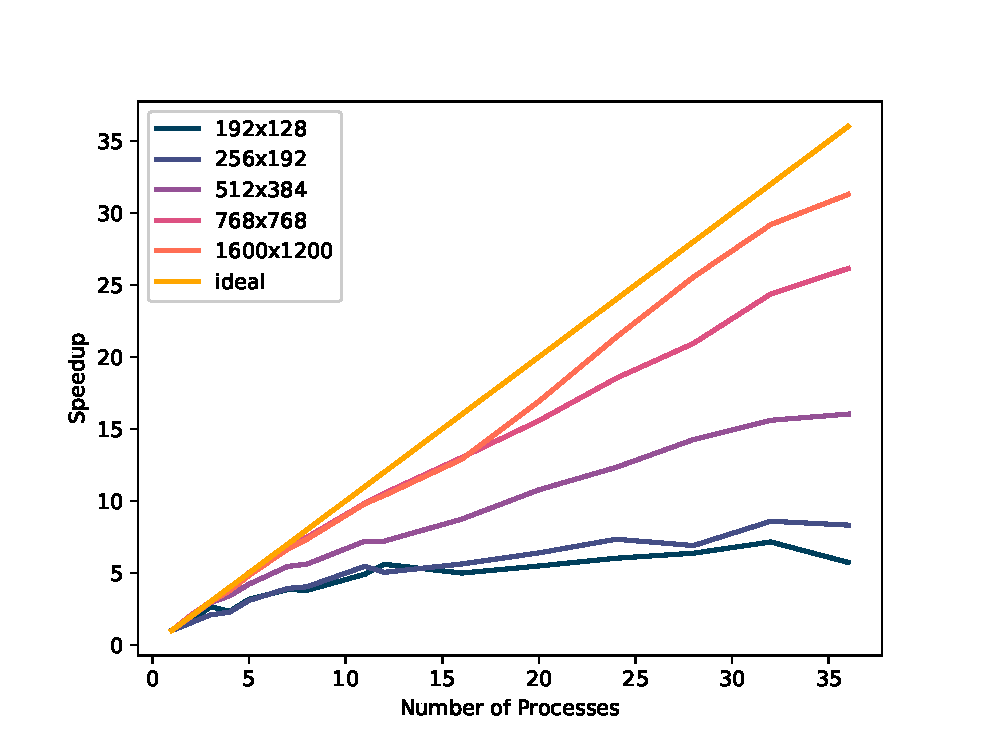
\includegraphics[scale=0.8]{../graphs/speedup.eps}
            \caption{Speedup for all the input images}
            \label{speedup}
          \end{figure}

          \paragraph{Small Input}
            Ideally as we increase the processors running the speedup should be increased accordingly but this is not the case for small problems. Let's take for example the case where the input image is 192x128 or 256x192 pixels. In Figure \ref{speedup}, it plain to see that the problem doen't scale as it should. When we use even more processors the speedup is slightly inclined. This possibly because the arithmetic calcluations consume a little amound of time as opposed to the halo swaps. As a result, for the specific size of problems 5 till 12 processes would be the best option. We don't have to waste 10 or 20 more of them if the speedup is not going to exceed 5 and 6 accrodingly.

          \paragraph{Medium Input}
            As long as we increase the input image size the speedup is growing faster. From Figure \ref{speedup} we can denote that for the image 512x384 choosing 26 processes seems a very appealing option. Reaching speedup 13 times faster than running it on one process.

          \paragraph{Big Input}
            In case of input size bigger than 768x768 pixels, the results are promising. Speedup is increased almost in a linear fashion, reaching the ideal values and making the communication overhead of the halo swaps to be insignificant. So we decided to do a further investigation and run the experiment for the big images with even more processes. In Figure \ref{speedupBigInput} we see the speedup results from 36 to 180 number of processes for the big input files. As expected, there is a point that each of the experiment's speedup is beginning to decline. It worth mentioning that to implement the specific experiment more that 1 nodes in Cirrus has been used. So the communication overhead is increased, due to network packages sending over the different nodes.

            \begin{figure}[h!]
              \centering
              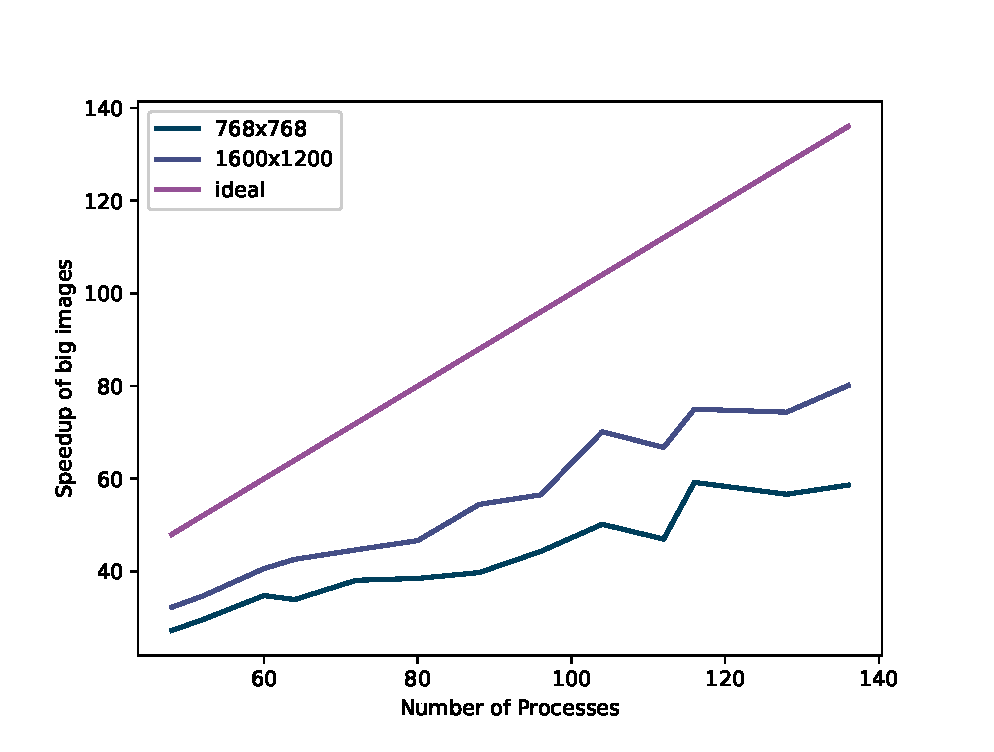
\includegraphics[scale=0.8]{../graphs/speedupBigInput.eps}
              \caption{Speedup for all big input images}
              \label{speedupBigInput}
            \end{figure}

          As a result we can certainly say that as long as the input size is increased the it comes to a point that Speedup starts to decline. Below in Table \ref{tableSpeedup} we have gathered for each input file a recommended number of processes in order to get a satisfing Speedup.

	      \begin{table}[h!]
	       \centering
	       \begin{tabular}{|p{3cm}||p{5cm}|p{3cm}|}
	         \hline
	         \multicolumn{3}{|c|}{Maximum Number of Processes} \\
	         \hline
	         Image size&Number of Processes&Speedup\\
	         \hline
	         192x128&12&4\\
	         256x192&26&7\\
	         512x384&26&12\\
	         768x768&84&27\\
	         1600x1200&-&-\\
	         \hline
	       \end{tabular}
	       \caption{Recommened Number of Processes and its Speedup}
	       \label{tableSpeedup}
	      \end{table}

        \subsubsection{Intervals}
          We made the design decision to print the average pixel and check the terminate condition every 100 iterations. That decision has been made in order to reduce the execution time. We made an experiment running for 1000 iterations the image 768x768 with and without intervals. In Figure \ref{speedupWithInterval} we can see adding this intervals change drastically the speedup of the experiment. 

          \begin{figure}[ht]
              \centering
              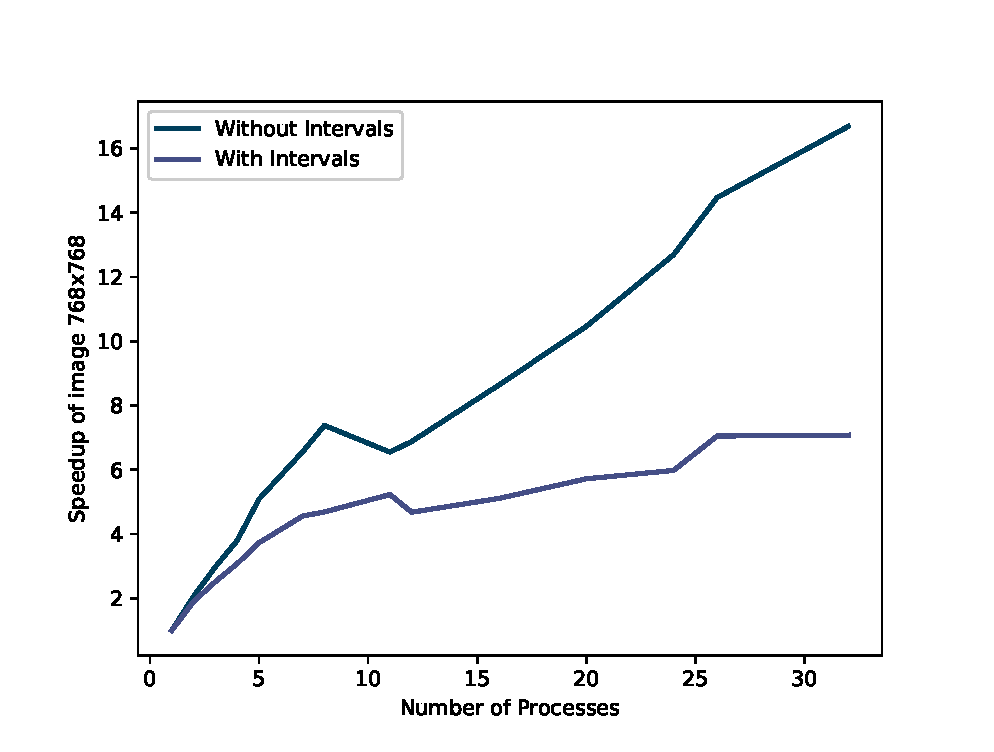
\includegraphics[scale=0.6]{../graphs/speedupInterval.eps}
              \caption{Speedup for all the input images}
              \label{speedupWithInterval}
          \end{figure}

        \subsubsection{Average Pixel}

        	In this section we have performed analysis regarding the average pixel results. Each iteration the average pixel is calculated. In order to achieve that we had to run the experiment till completion for all of the input images. We choose to run them once on 16 process, because the number of processes has not effect on the average pixel value. This happens due to the fact that the average pixel is depending on the input image and not in how many processes are participation on solving the problem.

        	\begin{figure}[ht]
    			  \centering
    				\subfloat[Average pixel for image 192x128]{{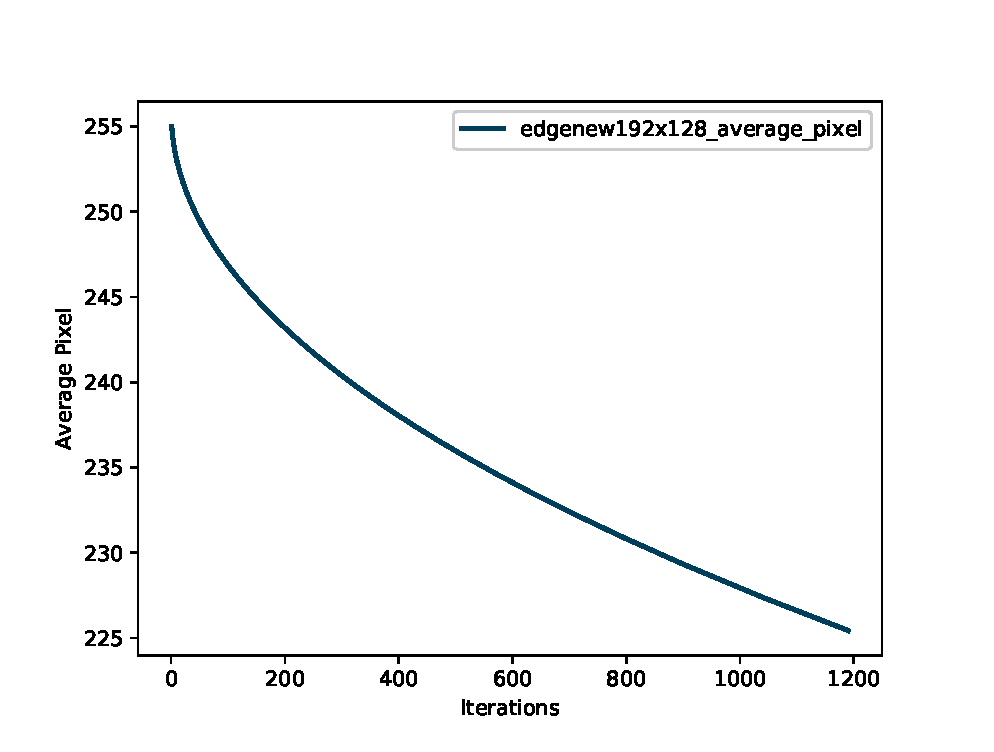
\includegraphics[width=.42\linewidth]{../graphs/average_pixel/edgenew192x128_average_pixel.eps} }}
  			    \qquad
  			    \subfloat[Average pixel for image 256x192]{{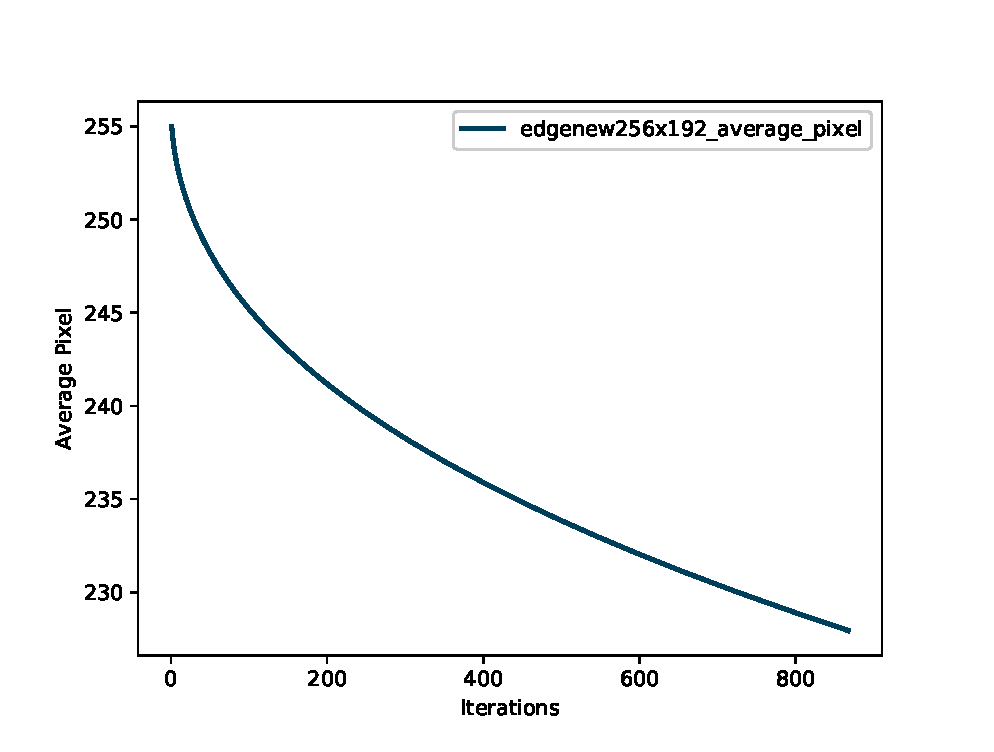
\includegraphics[width=.42\linewidth]{../graphs/average_pixel/edgenew256x192_average_pixel.eps} }}
  			    \qquad
  			    \subfloat[Average pixel for image 768x768]{{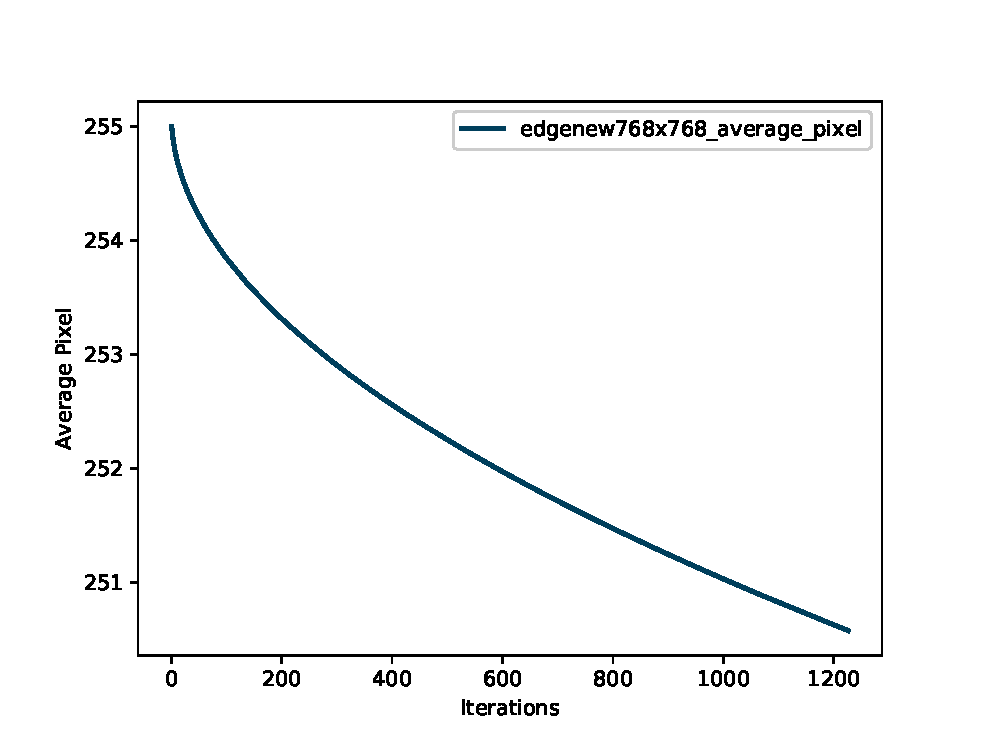
\includegraphics[width=.42\linewidth]{../graphs/average_pixel/edgenew768x768_average_pixel.eps} }}
  			    \qquad
  			    \subfloat[Average pixel for image 1600x1200]{{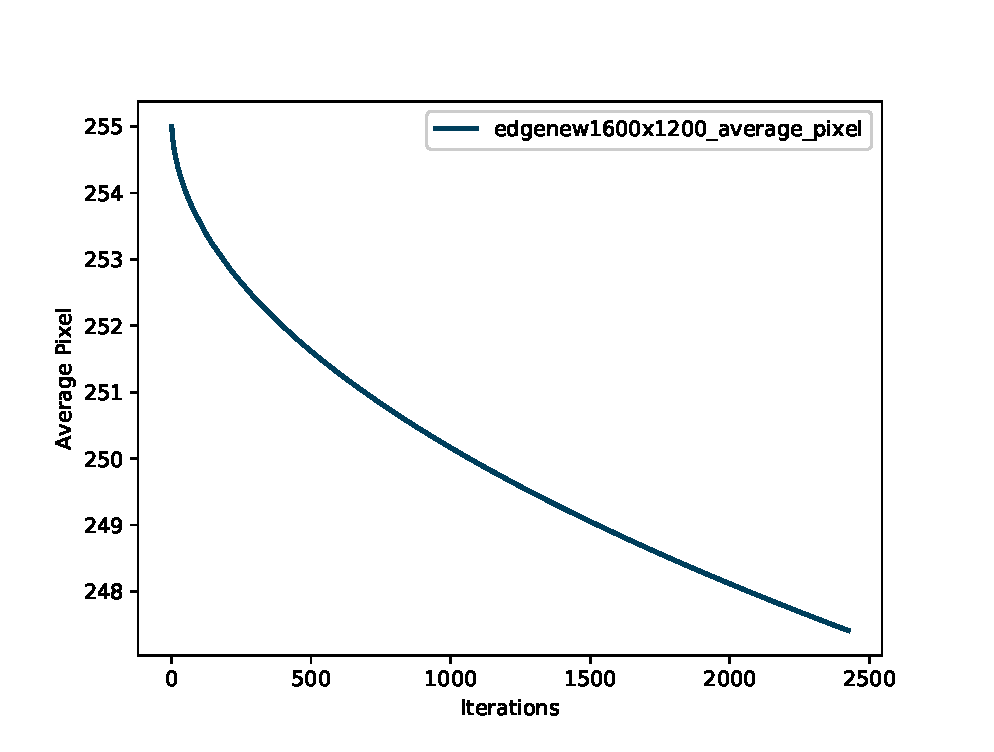
\includegraphics[width=.42\linewidth]{../graphs/average_pixel/edgenew1600x1200_average_pixel.eps} }}
  			    \caption{Average pixel for input images}
  			    \label{average_pixel}
    			\end{figure}

            According to Figure 2, which includes the average pixel values of 4 input images against the iteration number we can make some useful observations. First of all, the number of iterations is in some occasions independent of the size of the input image. This is because the number of iterations untill we can terminate the process is depending on how much easy is to reconstruct the specific image. For example, we can see doing a comparison in Figure 2 between  (a) and (b) that image 192x128 is indeed smaller than 256x192 but it takes 300 more iterations to be terminated.

            Secondly, it is plain to see that the average pixel's value is declined in every occassion. That observion is logical due to the fact that the initialized old buffer contain white (255) pixels. As long as the loop is processed the average value is decreasing, meaningly the whole picture is becoming darker. At this point, it worths to mention that in each image for the first iterations the pixel value is declined very fast. After that, the change rate is slower, meaning that each iteration has small impact to the new calculated output.

\sectionVspacing

\section{Conclusion}
	In conclusion, depending on the size of given problem the answer for the best approach to solve it, always varies. We could easily say that as long as the problem size is increased we have to do the same with the resources, in order to achieve the minimum running time. Indeed, if we want to exploit the best out of our system, further investigation is required. Luckily, this doesn't mean that we have to run our experiment until completion to identify the best approach. A small number of iterations of the main calculation loop are enough to identify the best suited system configurations. This choice is based on the experiment results, but always taking into account our available resources and budget, which is energy consumption and as always the given time.

\end{document}
